\begin{flushleft}
	\section{Vista de escenarios}

		La \textbf{vista de escenarios} (también conocida como \textit{vista +1} o \textit{vista de casos de uso}) es la quinta perspectiva del modelo de arquitectura 4+1. Esta vista no presenta una estructura estática por sí misma, sino que utiliza un conjunto de \textbf{casos de uso o escenarios representativos} para mostrar cómo los elementos definidos en las cuatro vistas principales (lógica, de procesos, de desarrollo y física) \textbf{interaccionan para satisfacer los requisitos del sistema}. Los escenarios describen secuencias de interacciones entre objetos y procesos, y sirven para:
		
		\begin{itemize}
			\item \textbf{Identificar y descubrir elementos arquitectónicos} durante el diseño.  
			\item \textbf{Validar e ilustrar} el diseño de la arquitectura una vez que está completo.  
			\item \textbf{Proveer narrativas concretas} que integran las otras vistas y facilitan la comunicación con los interesados.  
		\end{itemize}
		
		En esencia, la vista de escenarios actúa como \textbf{unificador y verificador} de las demás vistas del modelo 4+1, mostrando de forma práctica cómo funciona el sistema a través de ejemplos concretos de uso.
	\subsection{Diagrama de casos de uso}
	
	A continuación, se describen los \textbf{escenarios de la vista +1 (vista de escenarios)} basándose en la \textbf{Tabla 3.1 (Requerimientos Funcionales, pág. 39)} y en los \textbf{Requerimientos No Funcionales (pág. 41)}.
	
	\begin{figure}[H]
		\centering
		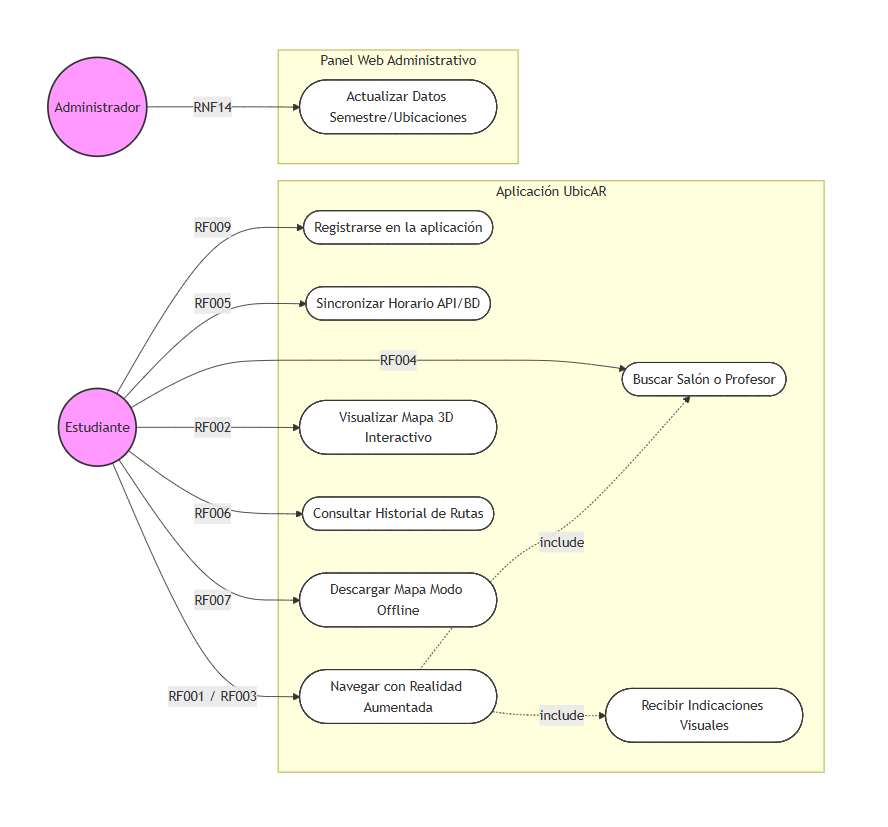
\includegraphics[width=0.95\textwidth]{imagenes/vista-escenarios.png}
		\caption{Vista de escenarios de la aplicación UbicAR}
		\label{fig:vista-escenarios}
	\end{figure}
	
	\newpage
	
	\subsection*{Actor: Estudiante}
	
	El \textbf{estudiante} es el usuario principal de la aplicación dentro de la UPIICSA. Sus escenarios clave son los siguientes:
	
	\begin{itemize}
		\item \textbf{Navegar con Realidad Aumentada (RF001, RF003, RF008):}  
		Es el escenario principal (\textit{Core}) del sistema. El estudiante selecciona un destino dentro del campus y la aplicación utiliza la cámara del dispositivo para detectar su ubicación en interiores, superponiendo flechas direccionales y elementos visuales en el entorno real para guiarlo hasta su destino.
		
		\item \textbf{Sincronizar Horario (RF005):}  
		El estudiante conecta la aplicación con su horario escolar. A partir de esta información, el sistema puede sugerir automáticamente a qué salón debe dirigirse según la hora y el día, reduciendo la necesidad de búsquedas manuales.
		
		\item \textbf{Buscar Salón o Profesor (RF004):}  
		El usuario ingresa manualmente el nombre de un profesor o el número de un aula, y el sistema calcula y muestra la ruta correspondiente dentro del campus.
		
		\item \textbf{Modo Offline (RF007):}  
		El estudiante descarga previamente los mapas y datos del semestre, lo que le permite utilizar la navegación y visualización del campus sin necesidad de conexión a internet.
		
		\item \textbf{Visualizar Mapa 3D (RF002):}  
		Como alternativa a la navegación con realidad aumentada, el estudiante puede consultar un mapa tridimensional del edificio, donde se muestra su posición y las rutas disponibles.
	\end{itemize}
	
	\subsection*{Actor: Administrador (Personal no técnico)}
	
	Este actor se identifica a partir del requerimiento \textbf{RNF14 (Actualización de Datos, pág. 41)}.
	
	\begin{itemize}
		\item \textbf{Actualizar Datos:}  
		Al inicio de cada semestre, los horarios, la ubicación de salones y los cubículos de los profesores pueden cambiar. El administrador utiliza un \textbf{panel web administrativo} para actualizar esta información sin requerir conocimientos técnicos ni la publicación de una nueva versión de la aplicación en las tiendas.
	\end{itemize}
	
	\subsection*{Justificación Arquitectónica (Modelo 4+1)}
	
	De acuerdo con lo establecido en las páginas 36 y 42 del documento, la \textbf{vista de escenarios} cumple las siguientes funciones:
	
	\begin{itemize}
		\item \textbf{Guiar el diseño de la arquitectura:}  
		Escenarios centrales como la \textit{Navegación con Realidad Aumentada} implican la necesidad de componentes de \textbf{visión por computadora} y frameworks de AR (por ejemplo, Vuforia o AR Foundation), los cuales se reflejan directamente en la \textbf{Vista Lógica}.
		
		\item \textbf{Validar la arquitectura propuesta:}  
		La correcta ejecución de escenarios como \textit{Sincronizar Horario} y \textit{Actualizar Datos} confirma que la \textbf{Vista de Datos} y la comunicación con el \textbf{Backend} (RNF10) están adecuadamente definidas y soportan los requerimientos del sistema.
	\end{itemize}
	

\end{flushleft}